\subsection{Meta Surfaces}

\subsection{The S-Matrix Formalism}

\begin{equation}
    \hat{S} =
    \begin{pmatrix}
        \hat{T}^f & \hat{R}^b \\
        \hat{R}^f & \hat{T}^b
    \end{pmatrix}
\end{equation}


\subsection{SASA and the Star Product}


\subsection{(Convolutional) Neural Networks}
Artificial Neural Networks (ANN's or short NN's) are a kind of data structure inspired by the biological Neurons found in Nature. They can be used to find a wide range of input output relations. One classic example is mapping pictures of hand written digits to the actual digits. Rather then explicitly program the relation NN's are trained on a dataset $(X, \, Y)$ of correct input output pairs.
\\


\begin{figure}[H]
    \centering
    \includegraphics[width=.6\linewidth]{bg_basic_nn}
    \caption{The most simple kind of NN is called densely connected. For clarity only connections to the top most nodes of each layer are shown.}
    \label{fig:bg:basic_nn}
\end{figure}

A NN consist of single nodes which are organized into layers where every node is connected to all the nodes of the previous and next layer. Each node holds a value called activation where the activation to the first layer is the input to the network, here:
$(x_1, \, x_2, \, x_3)$.
To calculate the activation of a node one has to multiply all the previous activations with their respective weights, add the bias and finally apply a non-linear activation function $\sigma$. For the example in \ref{fig:bg:basic_nn} that means:

\begin{equation}
    a = \sigma \qty(b + \sum_i w_i \, x_i)
\end{equation}
